\chapter*{\LaTeX Tutorial}

The following is an introduction to some of the basic utilities of \LaTeX. While this tutorial may not answer all of your questions, the good news is that \LaTeX is widely used enough that the answer is probably out there somewhere! If you need additional help, you can consult:

\begin{itemize}
    \item Claire Warner (\url{cwarner@roclefeller.edu}) at the Rita \& Frits Markus Library
    \item Google! The internet is your friend, and it's almost guaranteed that someone has already asked your question before (and someone else has provided a solution). You will likely find help on 
    \begin{itemize}
        \item StackExchange or StackOverflow
        
    \end{itemize}
\end{itemize}

\section{Sections, Subsections, and Sub-Subsections}

You may want to organize your dissertation text by using a section hierarchy within your chapters. Sections, subsections, and sub-subsections will be automatically translated into the Table of Contents. 

\subsection{Subsection}

This is a subsection.

\subsubsection{Sub-Subsection}

This is a sub-subsection.

\section{Citing References}

You can cite references throughout your thesis. \LaTeX makes this easy through the use of a .bib file. The file called \url{references.bib} is where you will put all of the citations that you would like to reference in the main text of your dissertation. The references are in BibTeX format within the .bib file. There are severaL ways to automatically format references in this style:

\begin{itemize}
    \item Use the Google Scholar Chrome extension. You can search for the desired article, click on ``Cite" and select the BibTeX option. This will open a tab of plain text that can be copied and pasted into the .bib file.
    \item Use citation management software and export the desired citation(s) in BibTeX format. Note that while Zotero and Mendeley will do this easily, EndNote can cause more problems and will not automatically generate convenient citation keys. Once you have exported the citations, copy the text into the .bib file or upload the new file (if you do this, be sure to change the .bib file referenced in the main \url{thesis.tex} file).
    \item Link your citation manager directly to Overleaf. You can use this feature with either Mendeley or Zotero.
\end{itemize}

Note that the references can be put into the .bib file in any order - they will automatically be formatted in the correct order when the References section is generated. To cite a reference in the text, simply type \url{\cite{key}}. Here, \url{key} is the citation key defined in the .bib entry for that citation. To cite multiple references at once, type \url{\cite{key1, key2}}. For example, \cite{ref1, ref2} and \cite{ref3} are the references selected for this tutorial.

References will be enumerated in order of the first time they are cited. Citing them later in the text will maintain this numbering scheme and show the original citation number, like so: \cite{ref1}.

\section{Acronyms and Abbreviations}

You can add acronyms to the main text by writing something like the following: \acrlong{dna} (abbreviated \acrshort{dna}) is the molecule that carries genetic information for the development and functioning of an organism. This will populate the referenced acronym into the List of Acronyms in the front matter of your dissertation. Note that you must add the acronym to the \url{Abbreviations.tex} file \textbf{and} refer to it in the main text by its defined tag for it to appear in the List of Acronyms. The acronyms/abbreviations will appear listed in alphabetical order. Note that the List of Acronyms is an optional component of your dissertation. If you do not include it, be sure to define any acronyms or abbreviations where necessary in the text for clarity.

\section{Footnotes}

Here is an example of how to use footnotes. It is possible to write footnotes directly in the text itself \footnote{By using the footnote command and writing your note in the curly brackets}. Or it is possible to mark the location of a footnote with footnote mark command\footnotemark \, then you can write the footnote in its own line for ease of reading. 

\footnotetext{You then use the footnotetext command and write your footnote as previously.}

\section{Figures and Tables}

Figures and tables are important ways of visualizing data and conveying information. As always, be sure to cite figures and tables if they are not your own work, or if they have been featured in previous publications. \LaTeX provides environments for both figures and tables. Within each environment, you can specify the image file (or table contents and layout) as well as the title and caption.

\subsection{Figures}

% This is a figure. Copy and paste this block of code for each figure. Change the width, image file path, title, and caption as needed. 
\begin{figure}
	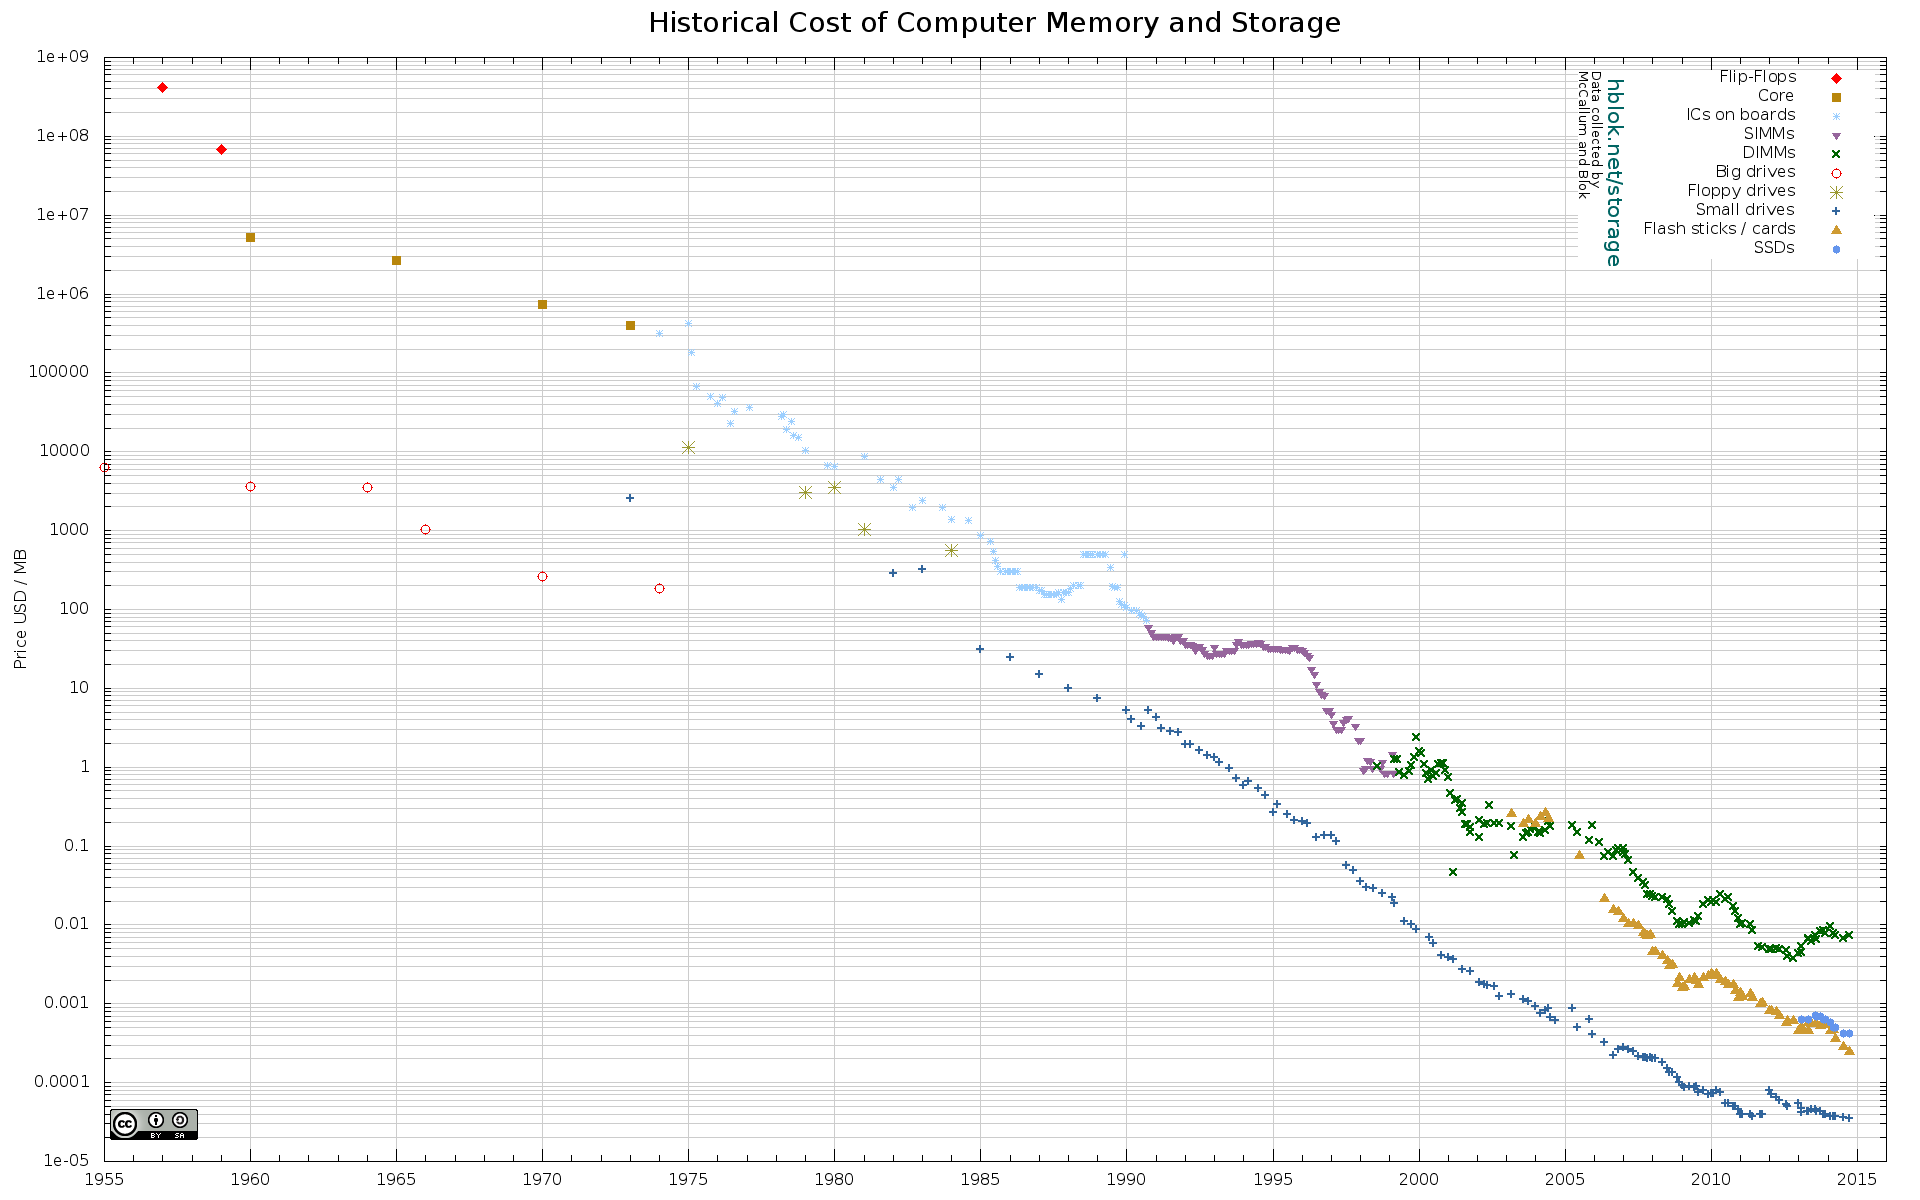
\includegraphics[width=\textwidth]{figures/exampleFigure.png} % Adjust width and file path as needed.
	\caption[Figure title for the Table of Contents]{ 
    Figure title for the main text. % By default, this should be identical to the figure title used in the Table of Contents.
    \textmd{Type a longer subtitle or caption here, optionally, which will appear unbolded in the main text.}
    }
	\label{figurelabel} % Refer to this figure in the main text by typing \ref{figurelabel}. Be sure to give each figure a unique and sensible label.
\end{figure}

You should try to include figures close to where they are discussed in the text. You can refer to any figure, such as Figure \ref{figurelabel}, in the text. Note that if you switch the order that figures are included in your \LaTeX code, the references in the text will automatically have their numbers updated, saving you a headache!

\subsection{Tables}

% This is a table
% Adapt the number of figures and columns as needed.
\begin{table}
\caption[Table title for the Table of Contents]{ 
    Table title for the main text. % By default, this should be identical to the figure title used in the Table of Contents.
    \textmd{Type a longer subtitle or caption here, optionally, which appears unbolded in the main text.}
    }\begin{center}
\begin{tabular}{ccc}
x & f(x) & g(x) \\
\hline
1 & 6 & 4  \\
2 & 6 & 3  \\
3 & 6 & 2  \\
4 & 6 & 2  \\
\label{Table in Chapter 1}
\end{tabular}
\end{center}
\end{table}

